\chapter{Analyses}

\label{ch:analysis}

Before designing an educational product, it is important that the designer first acquaints himself with the extrinsic factors important to this product. In order to discover the important characteristics of these factors, \citeA{instructionaldesign} enlist three types of analyses to be conducted, together with steps for conducting them. These are an analysis of the context, encompassing the needs of the users, and the environmental characteristics, an analysis of the learner, and an analysis of the learning task. Although these analyses are more targeted towards instructional design, and therefore more focused on a specific group being taught specific content, these analyses will still provide relevant information for the design choices and the evaluation. However, the steps will be adjusted and generalised or even omitted in order to fit the design of the more generic learning tool. The information gathered in order to conduct these analyses mainly stems from meetings with one of the teachers. This might not be the most reliable source of information because of the lack of triangulation, and should therefore not be taken as insight in the curriculum of Dutch Literature courses in secondary education, but rather as context information relevant to the design.

\section{Analysis of the learning context}

As already stated in the \nameref{sec:intro_evaluation} section on page~\pageref{sec:intro_evaluation}, the evaluation of the flashmap system will be evaluated within the Dutch secondary school Stedelijk Lyceum, with students having to learn about the Renaissance genres in Dutch Literature. This context will be further investigated within this section, starting with the Needs Assessment \cite{instructionaldesign}. Because although the general needs for a flashmap system are already described in the \nameref{ch:problem}, it is still important to investigate the specific needs of the context where the programm will be implemented.

\subsection{Needs assessment}

According to \citeA{instructionaldesign}, the first step in a needs assessment is to assess whether there is a problem, and what the nature is of the problem (see figure~\ref{fig:needsassessment}, mostly to identify the problem, but also in order to assess whether the innovation model or the discrepancy model applies for determining the needs. The first step is to assess whether there really is a problem in order to establish the general need. During the meetings, the teacher did confirm the need for better retention and comprehension of the content, and indicated that most of the time the students only learned the night before the exam in order to get a high (enough) grade and consequently forget everything again. This is not only wasteful of the effort of learning, but also causes problems when the knowledge becomes relevant again in the next chapter. The cause of this problem therefore definitely lies within the learning process, and could possibly be improved by the use of a flashcard or flashmap system, so it can be concluded that there is indeed a problem caused by learning, and it is thereby useful to proceed with the next phase of the assessment. Finally, \citeA{instructionaldesign} finally state that if there already exists instruction for the relevant learning goals, since if so than one has to proceed by using the discrepancy model, and otherwise by using the innovation model. The new tool is only there to enhance the current learning process by adding an additional activity, rather than adding new learning goals to an empty space in the curriculum. Thereby, from an instructional perspecticve, the flashcard or flashmap system is only an improvement of the currently existing instructional activities rather than a new innovation, and therefore the discrepancy model will be used.

\begin{figure}
    \centering
    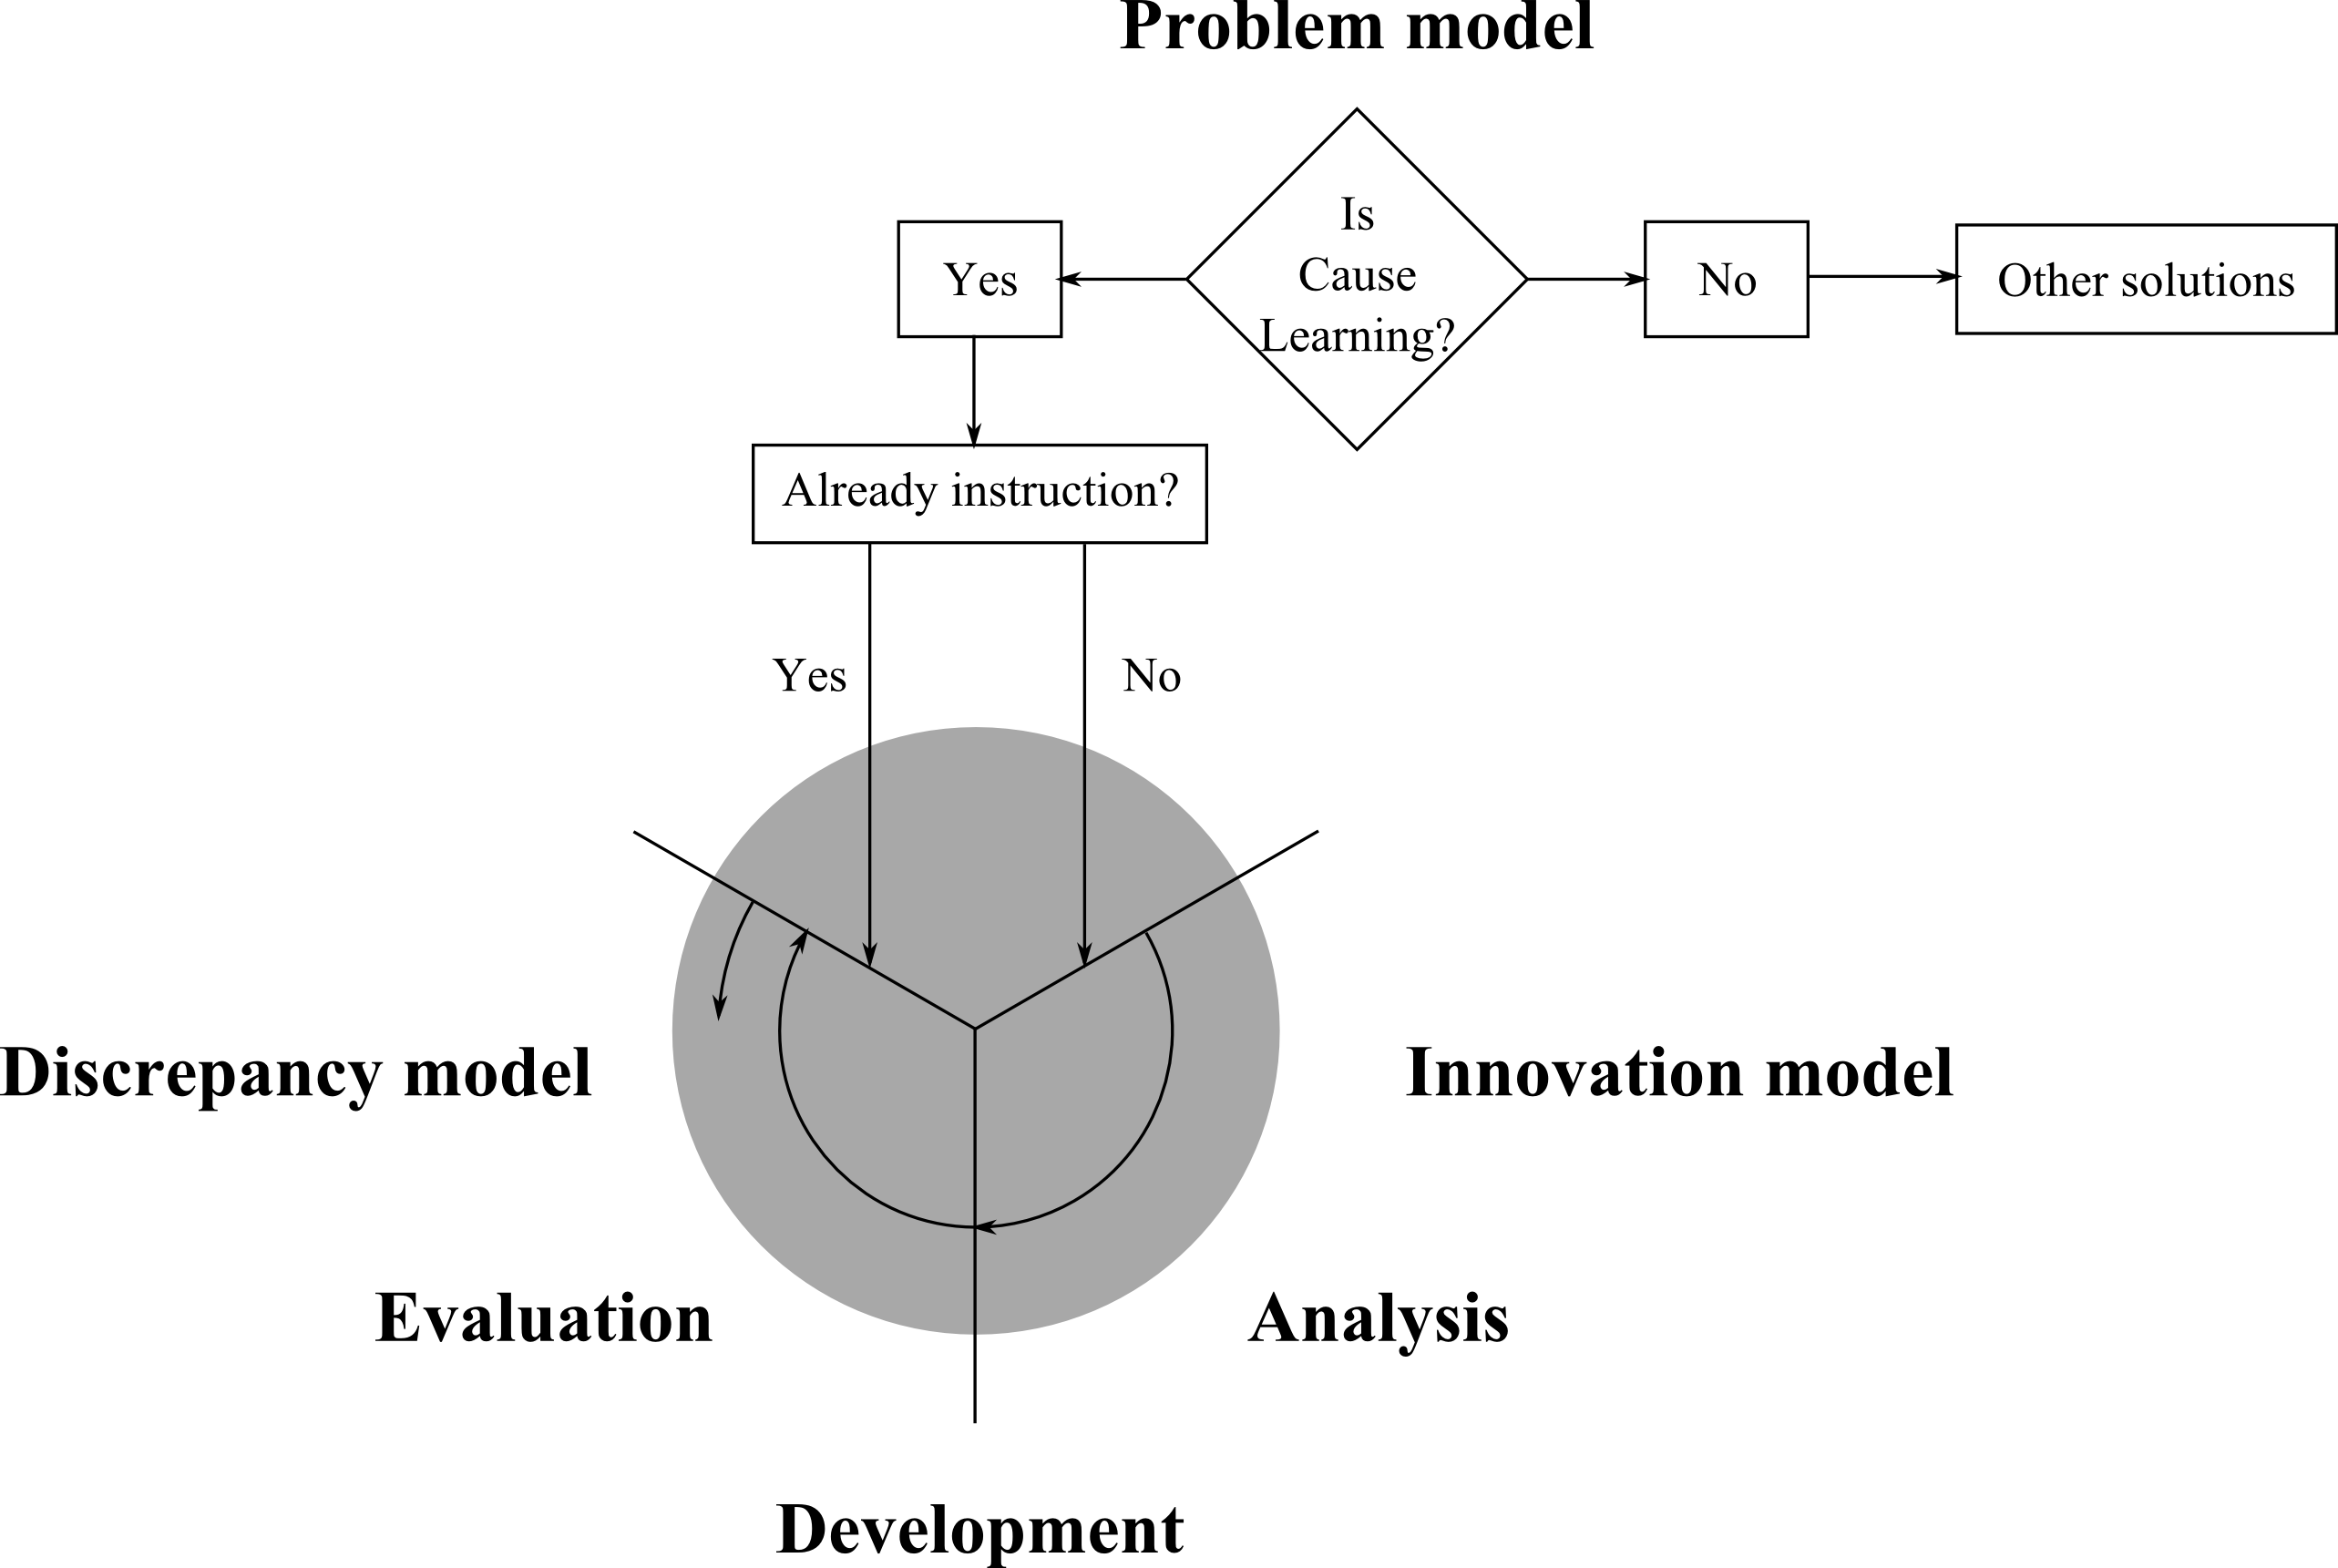
\includegraphics[width=\textwidth]{img/needsassessment.png}
    \caption{The three sides of needs assessment \protect\cite{instructionaldesign}}
    \label{fig:needsassessment}
\end{figure}

As can be seen in figure~\ref{fig:needsassessment}, the discrepancy model for needs assessment uses evaluative methods rather than analytical in order to establish the needs within the organisation. These methods include establishing the goals of the instructional system, determining how well these goals are currently being achieved, determining the gaps, prioritising the gaps, and determining which gaps are instructional needs (or in this case, educational needs). These remaining gaps can consecutively be used as a basis for determining the general use cases of the educational product. Normally an instructional designer tries to come into the organisation as a tabula rasa, without any preconceptions on what he would want to achieve and merely try to solve the real problem apparent in the organisation itself. However, because this design is theory driven rather than problem driven, it was merely checked with the teacher whether the problems stated in literature are also a problem here.

The first step was to confirm whether the goal stated by \citeA{glaserfield} of wanting students to memorise many facts in a meaningful way. Upon prompting the teacher what she deemed to be most important for her students to take away from her lessons was for them to become more familiar with the Dutch Renaissance writers or work. For example, she stated that she wanted the students to at least recognise important names when they saw a street name such as the "P.C. Hooftstraat" or the "Vondelpark". She also would like the students to be able to distinguish between different genres of literature, such as the \emph{sonnet} or \emph{emblematiek}. Based on these statements, the goals within the context are in line with students memorising and understanding all of the facts, without them being too ambitious. There are also differences between her and the other two teachers, they namely only offered the materials presented within the books, whereas she offered some additional content which the students also needed to master. However, she also stated that she would be responsible for the extra materials, and that the tool could be only to learn the textbook materials. Finally, she provided a test from the previous year to offer some more concrete examples of what she wanted the students to know, of which an English translation is included in the appendix on page~\pageref{ch:exampletest}.

\section{Analysis of the learner}

\section{Analysis of the task}
